\section{Schemata and plane models}

Consider the following picture:
\begin{center}
 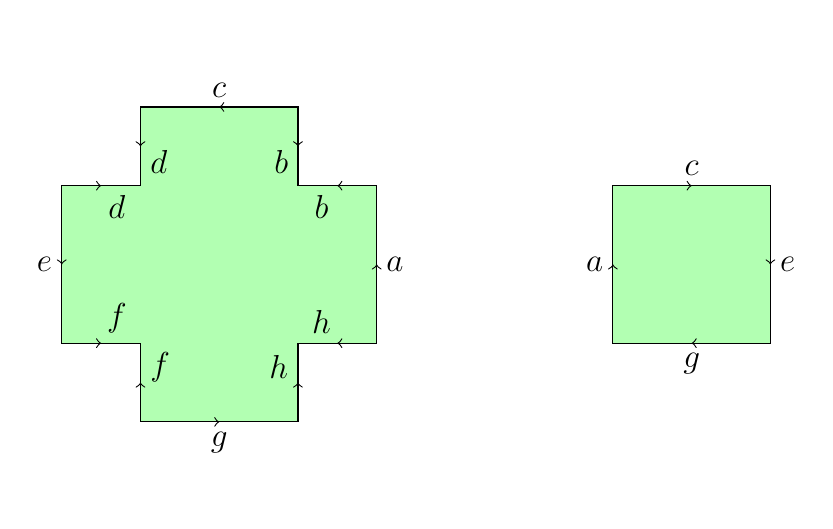
\begin{tikzpicture}
  \draw[white] (0, 3) -- (1, 3);
  \draw[white] (0,-3) -- (1,-3);
  \begin{scope}
   \filldraw[draw=black,fill=green!30]
    (2,-1) -- (2,1) -- (1,1) -- (1,2) -- (-1,2) -- (-1,1) -- (-2,1) --
    (-2,-1) -- (-1,-1) -- (-1,-2) -- (1,-2) -- (1,-1) -- (2,-1);
   \draw[black,->] ( 2.0,-1.0) -- ( 2.0, 0.0);
   \draw[black,->] ( 2.0, 1.0) -- ( 1.5, 1.0);
   \draw[black,->] ( 1.0, 2.0) -- ( 1.0, 1.5);
   \draw[black,->] ( 1.0, 2.0) -- ( 0.0, 2.0);
   \draw[black,->] (-1.0, 2.0) -- (-1.0, 1.5);
   \draw[black,->] (-2.0, 1.0) -- (-1.5, 1.0);
   \draw[black,->] (-2.0, 1.0) -- (-2.0, 0.0);
   \draw[black,->] (-2.0,-1.0) -- (-1.5,-1.0);
   \draw[black,->] (-1.0,-2.0) -- (-1.0,-1.5);
   \draw[black,->] (-1.0,-2.0) -- ( 0.0,-2.0);
   \draw[black,->] ( 1.0,-2.0) -- ( 1.0,-1.5);
   \draw[black,->] ( 2.0,-1.0) -- ( 1.5,-1.0);
   \draw[black] ( 2.0, 0.0) node[anchor=west ] {\large $a$};
   \draw[black] (-2.0, 0.0) node[anchor=east ] {\large $e$};
   \draw[black] ( 0.0, 2.0) node[anchor=south] {\large $c$};
   \draw[black] ( 0.0,-2.0) node[anchor=north] {\large $g$};
   \draw[black] ( 1.3, 1.0) node[anchor=north] {\large $b$};
   \draw[black] ( 1.0, 1.3) node[anchor=east ] {\large $b$};
   \draw[black] (-1.3, 1.0) node[anchor=north] {\large $d$};
   \draw[black] (-1.0, 1.3) node[anchor=west ] {\large $d$};
   \draw[black] (-1.3,-1.0) node[anchor=south] {\large $f$};
   \draw[black] (-1.0,-1.3) node[anchor=west ] {\large $f$};
   \draw[black] ( 1.3,-1.0) node[anchor=south] {\large $h$};
   \draw[black] ( 1.0,-1.3) node[anchor=east ] {\large $h$};
  \end{scope}
  \begin{scope}[xshift=6cm] 
   \filldraw[draw=black,fill=green!30] (-1,-1) rectangle (1,1);
   \draw[black,->] (-1.0,-1.0) -- (-1.0, 0.0);
   \draw[black,->] (-1.0, 1.0) -- ( 0.0, 1.0);
   \draw[black,->] ( 1.0, 1.0) -- ( 1.0, 0.0);
   \draw[black,->] ( 1.0,-1.0) -- ( 0.0,-1.0);
   \draw[black] (-1.0, 0.0) node[anchor=east ] {\large $a$};
   \draw[black] ( 1.0, 0.0) node[anchor=west ] {\large $e$};
   \draw[black] ( 0.0, 1.0) node[anchor=south] {\large $c$};
   \draw[black] ( 0.0,-1.0) node[anchor=north] {\large $g$};
  \end{scope}
 \end{tikzpicture}
\end{center}

This is an example of what we call a \emph{schema} (the plural is
\emph{schemata}).  It consists of one or more polygons, where each
edge of each polygon is marked with a label and a direction.  Each
polygon has no holes, and so is homeomorphic to a closed disc.  Each
label occurs precisely twice: there are two edges marked $a$, and two
edges marked $b$, and so on.

Given a schema $S$, we can construct a surface $|S|$ by gluing
together each pair of edges with corresponding labels, in the
direction indicated by the arrows.  If we were being more careful we
would have to explain exactly how to construct $|S|$ as a subset of
$\R^n$ with a linear surface triangulation.  However, we will instead
just explain one example.  With the schema shown above, we can first
glue together the two copies of $b$, the two copies of $d$, the two
copies of $f$ and the two copies of $h$.  This converts the left hand
polygon into a box with no lid, but the right hand polygon serves as
the lid, so we end up with the surface of a cube.  This in turn is
homeomorphic to a sphere.

\begin{definition}
 Let $X$ be a connected PL closed surface.  A \emph{plane model} for
 $X$ is a schema $S$ with only one polygon, such that $X$ is
 homeomorphic to $|S|$.
\end{definition}

\begin{example}
 We have plane models as follows:
 \begin{center}
  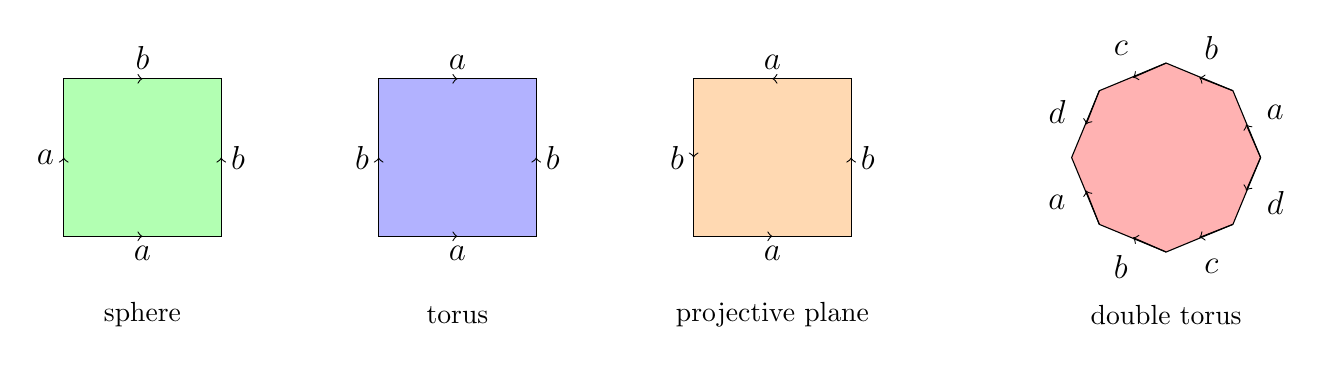
\begin{tikzpicture}
   \begin{scope}
    \filldraw[fill=green!30,draw=black] (0,0) rectangle (2,2);
    \draw[black,->] (0,0) -- (1,0);
    \draw[black,->] (2,0) -- (2,1);
    \draw[black,->] (0,0) -- (0,1);
    \draw[black,->] (0,2) -- (1,2);
    \draw[black] (1,0) node[anchor=north] {\large $a$};
    \draw[black] (0,1) node[anchor=east ] {\large $a$};
    \draw[black] (2,1) node[anchor=west ] {\large $b$};
    \draw[black] (1,2) node[anchor=south] {\large $b$};
    \draw[black] (1,-1) node{sphere};
   \end{scope}
   \begin{scope}[xshift=4cm]
    \filldraw[fill=blue!30,draw=black] (0,0) rectangle (2,2);
    \draw[black,->] (0,0) -- (1,0);
    \draw[black,->] (2,0) -- (2,1);
    \draw[black,->] (0,0) -- (0,1);
    \draw[black,->] (0,2) -- (1,2);
    \draw[black] (1,0) node[anchor=north] {\large $a$};
    \draw[black] (0,1) node[anchor=east ] {\large $b$};
    \draw[black] (2,1) node[anchor=west ] {\large $b$};
    \draw[black] (1,2) node[anchor=south] {\large $a$};
    \draw[black] (1,-1) node{torus};
   \end{scope}
   \begin{scope}[xshift=8cm]
    \filldraw[fill=orange!30,draw=black] (0,0) rectangle (2,2);
    \draw[black,->] (0,0) -- (1,0);
    \draw[black,->] (2,0) -- (2,1);
    \draw[black,->] (0,2) -- (0,1);
    \draw[black,->] (2,2) -- (1,2);
    \draw[black] (1,0) node[anchor=north] {\large $a$};
    \draw[black] (0,1) node[anchor=east ] {\large $b$};
    \draw[black] (2,1) node[anchor=west ] {\large $b$};
    \draw[black] (1,2) node[anchor=south] {\large $a$};
    \draw[black] (1,-1) node{projective plane};
   \end{scope}
   \begin{scope}[xshift=14cm,yshift=1cm]
    \filldraw[fill=red!30,draw=black]
     (0:1.2) -- (45:1.2) -- (90:1.2) -- (135:1.2) -- (180:1.2) -- (225:1.2) -- (270:1.2) -- (315:1.2) -- (0:1.2);
    \draw[black,->] (   0:1.2) -- (  22.5:1.1);
    \draw[black,->] (  45:1.2) -- (  67.5:1.1);
    \draw[black,->] (  90:1.2) -- ( 112.5:1.1);
    \draw[black,->] ( 135:1.2) -- ( 157.5:1.1);
    \draw[black,->] (   0:1.2) -- ( -22.5:1.1);
    \draw[black,->] ( -45:1.2) -- ( -67.5:1.1);
    \draw[black,->] ( -90:1.2) -- (-112.5:1.1);
    \draw[black,->] (-135:1.2) -- (-157.5:1.1);
    \draw[black] ( 22.5:1.5) node {\large $a$};
    \draw[black] ( 67.5:1.5) node {\large $b$};
    \draw[black] (112.5:1.5) node {\large $c$};
    \draw[black] (157.5:1.5) node {\large $d$};
    \draw[black] (202.5:1.5) node {\large $a$};
    \draw[black] (247.5:1.5) node {\large $b$};
    \draw[black] (292.5:1.5) node {\large $c$};
    \draw[black] (337.5:1.5) node {\large $d$};
    \draw[black] (0,-2) node{double torus};
   \end{scope}
  \end{tikzpicture}
 \end{center}
 The first two of these are not hard to understand.  The remaining two
 will be discussed in more detail later.
\end{example}

In this section, we will show that every PL closed surface has a plane
model.  In later sections we will show how plane models can be
simplified to a minimal form, and use that form to classify all
possible closed surfaces.

\begin{proposition}\label{prop-schema-exists}
 Let $X$ be a PL closed surface.  Then there is a schema $S$ such that
 $X$ is homeomorphic to $|S|$.
\end{proposition}
\begin{proof}
 Choose a linear surface triangulation of $X$, consisting of triangles
 $T_1,\dotsc,T_N$ and edges $E_1,\dotsc,E_M$.  We can then take $N$
 disjoint triangles $T'_1,\dotsc,T'_N$ in $\R^2$.  If the $i$'th edge
 of $T_p$ is $E_q$, then we mark the $i$'th edge of $T'_p$ with $q$.
 This gives a schema $S$, and it is not hard to see that $|S|=X$.
\end{proof}

A key technique in the theory of surfaces is to start with a schema
$S$ and somehow produce a simpler schema $T$ with $|T|\simeq|S|$.  As
a basic example, we can simplify the above schema by gluing together
the two copies of $a$.  This converts $a$ to an internal edge, which
we can harmlessly erase.  The resulting schema is as follows:
\begin{center}
 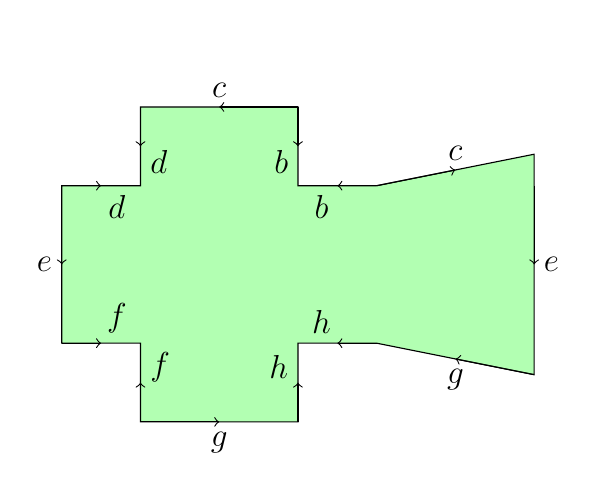
\begin{tikzpicture}
  \draw[white] (0,3) -- (1,3);
  \begin{scope}
   \filldraw[draw=black,fill=green!30]
    (2,1) -- (1,1) -- (1,2) -- (-1,2) -- (-1,1) -- (-2,1) --
    (-2,-1) -- (-1,-1) -- (-1,-2) -- (1,-2) -- (1,-1) -- (2,-1) --
    (4,-1.4) -- (4,1.4) -- (2,1);
   \draw[black,->] ( 2.0, 1.0) -- ( 1.5, 1.0);
   \draw[black,->] ( 1.0, 2.0) -- ( 1.0, 1.5);
   \draw[black,->] ( 1.0, 2.0) -- ( 0.0, 2.0);
   \draw[black,->] (-1.0, 2.0) -- (-1.0, 1.5);
   \draw[black,->] (-2.0, 1.0) -- (-1.5, 1.0);
   \draw[black,->] (-2.0, 1.0) -- (-2.0, 0.0);
   \draw[black,->] (-2.0,-1.0) -- (-1.5,-1.0);
   \draw[black,->] (-1.0,-2.0) -- (-1.0,-1.5);
   \draw[black,->] (-1.0,-2.0) -- ( 0.0,-2.0);
   \draw[black,->] ( 1.0,-2.0) -- ( 1.0,-1.5);
   \draw[black,->] ( 2.0,-1.0) -- ( 1.5,-1.0);
   \draw[black] (-2.0, 0.0) node[anchor=east ] {\large $e$};
   \draw[black] ( 0.0, 2.0) node[anchor=south] {\large $c$};
   \draw[black] ( 0.0,-2.0) node[anchor=north] {\large $g$};
   \draw[black] ( 1.3, 1.0) node[anchor=north] {\large $b$};
   \draw[black] ( 1.0, 1.3) node[anchor=east ] {\large $b$};
   \draw[black] (-1.3, 1.0) node[anchor=north] {\large $d$};
   \draw[black] (-1.0, 1.3) node[anchor=west ] {\large $d$};
   \draw[black] (-1.3,-1.0) node[anchor=south] {\large $f$};
   \draw[black] (-1.0,-1.3) node[anchor=west ] {\large $f$};
   \draw[black] ( 1.3,-1.0) node[anchor=south] {\large $h$};
   \draw[black] ( 1.0,-1.3) node[anchor=east ] {\large $h$};
  \end{scope}
  \begin{scope}[xshift=3cm] 
   \draw[black,->] (-1.0, 1.0) -- ( 0.0, 1.2);
   \draw[black,->] ( 1.0, 1.0) -- ( 1.0, 0.0);
   \draw[black,->] ( 1.0,-1.4) -- ( 0.0,-1.2);
   \draw[black] ( 1.0, 0.0) node[anchor=west ] {\large $e$};
   \draw[black] ( 0.0, 1.2) node[anchor=south] {\large $c$};
   \draw[black] ( 0.0,-1.2) node[anchor=north] {\large $g$};
  \end{scope}
 \end{tikzpicture}
\end{center}

This can be done more generally:
\begin{proposition}\label{prop-model-exists}
 Let $S$ be any schema such that $|S|$ is connected.  Then there is
 another schema $T$ such that $T$ has only one polygon, and
 $|T|\simeq |S|$.
\end{proposition}
\begin{proof}
 Choose any polygon $P$ in $S$.  If $P$ shares a label with some other
 polygon $Q$, then we can choose one such label and glue the
 corresponding edges.  As we have only glued one pair of edges, it is
 easy to see that the result is still a polygon.  We can repeat this
 process until we have a schema $S'$ with a polygon $P'$ such that
 $P'$ shares no labels with any other polygon.  This means that $P'$
 is a schema by itself, as is $S'\sm P'$, and $|S'|$ is the disjoint
 union of $|P'|$ and $|S'\sm P'|$.  However, $|S'|$ is homeomorphic to
 $|S|$ and so is still be connected.  This can only be consistent if
 $P'$ is all of $S'$, and so $S'\sm P'$ is empty.
\end{proof}

\begin{corollary}
 Every PL closed surface has a plane model.
\end{corollary}
\begin{proof}
 Let $X$ be a PL closed surface.  Proposition~\ref{prop-schema-exists}
 tells us that there is a schema $S$ with $|S|\simeq X$.  Then 
 Proposition~\ref{prop-model-exists} tells us that we can find another
 schema $T$ with only one polygon such that $|T|\simeq |S|\simeq X$,
 so $T$ is a plane model for $X$.
\end{proof}

\end{document}
